\documentclass[11pt]{article}
\usepackage{graphicx}
\usepackage{hyperref}
%\usepackage{appendix}
\usepackage{amsmath}
\usepackage{amsthm}
\usepackage{amssymb}
\usepackage{float}
\usepackage{commath}
\usepackage{booktabs}
\renewcommand{\arraystretch}{1.2}
\usepackage{siunitx}
\sisetup{detect-all}
\usepackage{listings}
\usepackage{color} %red, green, blue, yellow, cyan, magenta, black, white
\definecolor{mygreen}{RGB}{28,172,0} % color values Red, Green, Blue
\definecolor{mylilas}{RGB}{170,55,241}
\usepackage[a4paper,margin=20mm]{geometry}
\numberwithin{equation}{section}
\setlength{\parskip}{\baselineskip}
\setlength{\parindent}{0pt}
\hypersetup{
    colorlinks=true,
    linkcolor=magenta,
    filecolor=magenta,      
    urlcolor=magenta,
}
\urlstyle{same}
\begin{document}
\title{\textbf{UCL Mechanical Engineering 2020/2021}\\ENGF0004 Coursework 2}
\author{NCWT3}
\maketitle
\section{Question 1}
\subsection{a}
For the line integral to be independent from the path of integration, the following conditions must be fulfilled:
\begin{gather}
    I = \int_A^B \left(\frac{\partial u}{\partial x} \dif x + \frac{\partial u}{\partial y}\dif y\right)\\
    P\left(x, \, y\right) = \frac{\partial u}{\partial x} \textrm{ and } Q\left(x, \, y\right) = \frac{\partial u}{\partial y}\\
    \frac{\partial P\left(x, \, y\right)}{\partial y} = \frac{\partial Q\left(x, \, y\right)}{\partial x}
\end{gather}
Considering the integral:
\begin{gather}
    I = \int_A^B \left[e^{-\alpha xy} \left(\frac{\alpha-2}{x}\right)\dif x - \frac{1}{\alpha y}\left(e^{-\alpha x y}-1\right)\dif y\right]\\
    P\left(x, \, y\right) = e^{-\alpha xy} \left(\frac{\alpha-2}{x}\right) \textrm{ and } Q\left(x, \, y\right) = - \frac{1}{\alpha y}\left(e^{-\alpha x y}-1\right)\\
    \frac{\partial P\left(x, \, y\right)}{\partial y} = -\alpha x \left(\frac{\alpha -2}{x}\right) e^{-\alpha xy} = \left(2\alpha - \alpha^2\right)e^{-\alpha xy}\\
    \frac{\partial Q\left(x, \, y\right)}{\partial x} = -\frac{1}{\alpha y}\left(-\alpha y\right)e^{-\alpha xy} = e^{-\alpha xy}\\
    \therefore 2\alpha e^{-\alpha xy} - \alpha^2 e^{-\alpha xy} = e^{-\alpha xy}\\
    e^{-\alpha xy} \left(\alpha^2 - 2\alpha + 1\right) = 0\\
    e^{-\alpha xy} = 0 \rightarrow \textrm{no solutions}\\
    \left(\alpha - 1\right)^2 = 0\\
    \alpha = 1
\end{gather}
\subsection{b}
Calculating the line integral of \ref{1beq1} from $O\left(0, \, 0\right)$ to $A(1, \, e-1)$ along $y=e^x -1$:
\begin{gather}
    I = \int_O^A \left(ye^{-2x}\right)\left(\dif x + \dif y\right) \label{1beq1}\\
    y = e^x - 1\\
    \dif y = e^x \dif x\\
    I = \int_0^1 \left( \left( e^x-1\right) \left( e^{-2x} \right) + \left( e^x-1\right)\left( e^{-2x}\right)\left( e^x\right)\right)\dif x \\
    = \int_0^1 \left(e^{-x} - e^{-x} - e^{-2x} +1\right)\dif x\\
    = \int_0^1 \left(1-e^{-2x}\right)\dif x \\
    = \left[x + \frac{e^{-2x}}{2}\right]_0^1\\
    = 1 + \frac{e^{-2}}{2} -0-\frac{1}{2}\\
    I = \frac{1}{2}\left(e^{-2}+1\right)
\end{gather}
\subsection{c}
\subsubsection{i}
Calculating $\nabla \cdot \underline{F}$:
\begin{gather}
    \underline{F}\left(x, \, y, \, z\right) = \begin{pmatrix}
        \frac{y}{x^2}\\
        \frac{x}{y^2}
    \end{pmatrix}\\
    \nabla \cdot \underline{F} = \begin{pmatrix}
        \frac{\partial}{\partial x}\\
        \frac{\partial}{\partial y}
    \end{pmatrix} \cdot \begin{pmatrix}
        \frac{y}{x^2}\\
        \frac{x}{y^2}
    \end{pmatrix}\\
    = \frac{\partial}{\partial x}\left(\frac{y}{x^2}\right) + \frac{\partial}{\partial y} \left(\frac{x}{y^2}\right)\\
    = -\frac{2y}{x^3}-\frac{2x}{y^3} \\
    = -2\left(\frac{y}{x^3}+\frac{x}{y^3}\right)
\end{gather}
\subsubsection{ii}
Calculating the double integral:
\begin{gather}
    I = \int_{1}^{2} \int_{1}^{2} \left(-2\left(\frac{y}{x^3}+\frac{x}{y^3}\right)\right) \dif x \dif y\\
    = \int_{1}^{2} \left[-2\left(\frac{y}{-2x^2} + \frac{x^2}{2y^3}\right)\right]_1^2 \dif y\\
    = \int_{1}^{2} \left[-2\left(-\frac{y}{8} + \frac{2}{y^3}+\frac{y}{2} - \frac{1}{2y^3}\right)\right] \dif y\\
    = \int_{1}^{2} \left(-\frac{3y}{4}-\frac{3}{y^3}\right) \dif y\\
    = \left[-\frac{3y^2}{8}+\frac{3}{2y^2}\right]_1^2\\
    = -\frac{3}{2} + \frac{3}{8} + \frac{3}{8} - \frac{3}{2}\\
    I = -\frac{9}{4}
\end{gather}
\subsection{d}
\subsubsection{i}
Calculating the line integral along the red path:
\begin{gather}
    I = \int \left(\sin x \cos y \dif y + \cos x \sin y \dif y\right)\\
    y = 0 \hspace{1cm} \dif y = 0\\
    I_{AB} = \int_{x=0}^{\pi} \left(\sin x\right)\dif x = \left[-\cos x\right]_0^{\pi} = 2\\
    x = \pi \hspace{1cm} \dif x = 0\\
    I_{BC} = \int_{y=0}^{\pi} \left(-\sin y\right)\dif y= \left[\cos y\right]_0^{\pi} = -2\\
    \therefore I = I_{AB} + I_{BC} = 2-2 = 0
\end{gather}
\subsubsection{ii}
Calculating the line integral along the blue path:
\begin{gather}
    I = \int \left(\sin x \cos y \dif y + \cos x \sin y \dif y\right)\\
    y = x \hspace{1cm} \dif y = \dif x\\
    I_{AC} = \int_0^{\pi} \left(\sin x \cos x + \sin x \cos x\right) \dif x\\
    = \int_0^{\pi} \left(\sin \left(2x\right)\right)\dif x\\
    I_{AC} = \left[-\frac{1}{2}\cos \left(2x\right)\right]_0^{\pi} = \frac{1}{2} - \frac{1}{2} = 0\\
\end{gather}
\subsection{e}
\subsubsection{i}
\begin{figure}[H]
    \centering
    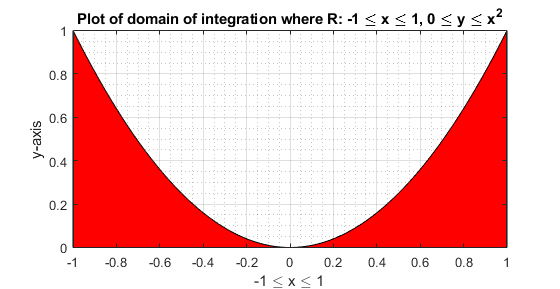
\includegraphics[width = 0.75 \textwidth]{./img/q1ei.png}
    \caption{Domain of integration where $R: \, -1 \leq x \leq 1, \, 0 \leq y \leq x^2$.}
\end{figure}
\lstset{language=Matlab,%
    %basicstyle=\color{red},
    breaklines=true,%
    morekeywords={matlab2tikz},
    keywordstyle=\color{blue},%
    morekeywords=[2]{1}, keywordstyle=[2]{\color{black}},
    identifierstyle=\color{black},%
    stringstyle=\color{mylilas},
    commentstyle=\color{mygreen},%
    showstringspaces=false,%without this there will be a symbol in the places where there is a space
    numbers=left,%
    numberstyle={\tiny \color{black}},% size of the numbers
    numbersep=9pt, % this defines how far the numbers are from the text
    emph=[1]{for,end,break},emphstyle=[1]\color{red}, %some words to emphasise
    %emph=[2]{word1,word2}, emphstyle=[2]{style},    
}
\lstinputlisting{./bin/q1ei.m}
\subsubsection{ii}
$y =0 \rightarrow y = x^2$ and $x = -1 \rightarrow x = 1 $
\begin{gather}
    I = \int_{-1}^{1} \int_{0}^{x^2} \left( y \frac{\sin\left(\pi x\right)}{x} \right) \dif y \dif z\\
    I = \int_{-1}^{1} \left[y^2 \frac{\sin\left(\pi x\right)}{2x}\right]_0^{x^2} \dif x\\
    I = \int_{-1}^{1} \left[\frac{x^4 \sin\left(\pi x \right)}{2x} - 0 \right] \dif x\\
    I = \int_{-1}^{1} \left(\frac{x^3 \sin\left(\pi x \right)}{2} \right) \dif x
\end{gather}
Integration by parts thrice: 
\begin{gather}
    u_x = \frac{x^3}{2} \hspace{1cm} u_x' = \frac{3x^2}{2}\\
    v_x = -\frac{\cos \left(\pi x\right)}{\pi} \hspace{1cm} v_x' = \sin \left(\pi x \right)\\
    I = \left[-\frac{x^3 \cos\left(\pi x\right)}{2\pi}\right]_{-1}^1 + \int_{-1}^1 \left(\frac{3x^2 \cos\left(\pi x\right)}{2\pi}\right) \dif x\\
    u_x = \frac{3x^2}{2\pi} \hspace{1cm} u_x' = \frac{3x}{\pi}\\
    v_x = \frac{\sin \left(\pi x\right)}{\pi} \hspace{1cm} v_x' = \cos \left(\pi x \right)\\
    I = - \frac{\cos \pi}{2\pi} - \frac{\cos(-\pi)}{2\pi} + \left[\frac{3x^2 \sin\left(\pi x\right)}{2x^2}\right]_{-1}^1 - \int_{-1}^1 \left(\frac{3x \sin\left(\pi x \right)}{\pi^2} \right) \dif x\\
    I = \frac{1}{2\pi} + \frac{1}{2\pi} + 0 - 0 - \int_{-1}^1 \left(\frac{3x \sin\left(\pi x \right)}{\pi^2} \right) \dif x\\
    u_x = \frac{3x}{\pi^2} \hspace{1cm} u_x' = \frac{3}{\pi^2}\\
    v_x = -\frac{\cos \left(\pi x\right)}{\pi} \hspace{1cm} v_x' = \sin \left(\pi x \right)\\
    I = \frac{1}{\pi} + \left[\frac{3x\cos\left(\pi x \right)}{\pi^3}\right]_{-1}^1 - \int_{-1}^1 \left(\frac{3\cos\left(\pi x\right)}{\pi^3}\right) \dif x\\
    I = \frac{1}{\pi} - \frac{3}{\pi^3} - \frac{3}{\pi^3} - \left[ \frac{3\sin\pi}{\pi^4} - \frac{3\sin(-\pi)}{\pi^4}\right]\\
    I = \frac{1}{\pi} - \frac{6}{\pi^3} = 0.125
\end{gather}
\subsubsection{iii}
Utilising symmetry, we can select the limits $x = 0, \, x=1$ and then multiply the result by 2:
\begin{align}
    I &= 2\int_0^1 \int_{\sqrt{y}}^1 \left(x^2 + y^2\right) \dif x \dif y\\
    &= 2\int_0^1 \left[\frac{x^3}{3} + xy^2\right]_{\sqrt{y}}^1 \dif y\\
    &= 2\int_0^1 \left(\frac{1}{3} + y^2 - \frac{y^{\frac{3}{2}}}{3} - y^{\frac{5}{2}}\right) \dif y\\
    &= 2\left[\frac{y}{3} + \frac{y^3}{3} - \frac{2y^{\frac{5}{2}}}{15} - \frac{2y^{\frac{7}{2}}}{7}\right]_0^1\\
    &= 2\left[\frac{1}{3} + \frac{1}{3} - \frac{2}{15} - \frac{2}{7}\right]\\
    I &= \frac{2\cdot 26}{105} = \frac{52}{105}
\end{align}
\subsection{f}
\subsubsection{i}
\begin{figure}[H]
    \centering
    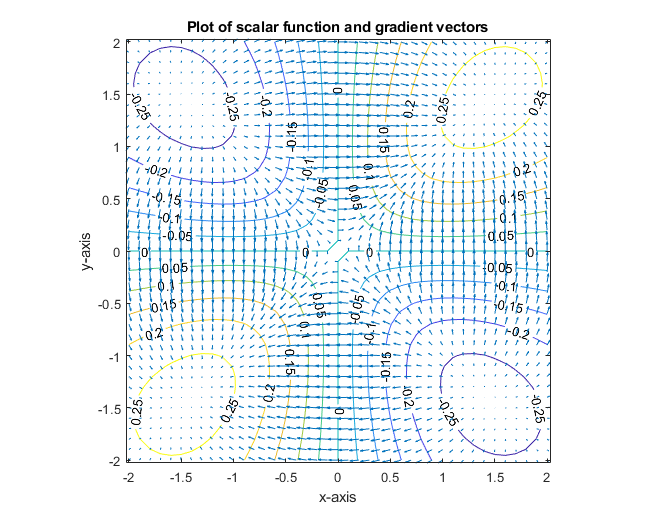
\includegraphics[width = 0.75 \textwidth]{./img/q1fi.png}
    \caption{Plot of scalar function $z= xye^{-\sqrt{x^2 + y^2}}$ and its gradient.}
\end{figure}
\lstset{language=Matlab,%
    %basicstyle=\color{red},
    breaklines=true,%
    morekeywords={matlab2tikz},
    keywordstyle=\color{blue},%
    morekeywords=[2]{1}, keywordstyle=[2]{\color{black}},
    identifierstyle=\color{black},%
    stringstyle=\color{mylilas},
    commentstyle=\color{mygreen},%
    showstringspaces=false,%without this there will be a symbol in the places where there is a space
    numbers=left,%
    numberstyle={\tiny \color{black}},% size of the numbers
    numbersep=9pt, % this defines how far the numbers are from the text
    emph=[1]{for,end,break},emphstyle=[1]\color{red}, %some words to emphasise
    %emph=[2]{word1,word2}, emphstyle=[2]{style},    
}
\lstinputlisting{./bin/q1fi.m}
\subsubsection{ii}
\begin{figure}[H]
    \centering
    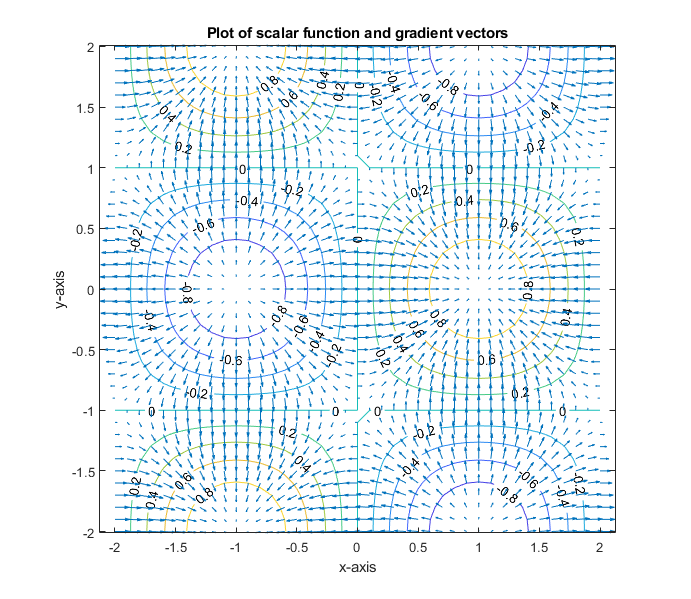
\includegraphics[width = 0.75 \textwidth]{./img/q1fii.png}
    \caption{Plot of scalar function $z= \sin\left(\frac{\pi}{2}x\right)\cos\left(\frac{\pi}{2}y\right)$ and its gradient.}
\end{figure}
\lstset{language=Matlab,%
    %basicstyle=\color{red},
    breaklines=true,%
    morekeywords={matlab2tikz},
    keywordstyle=\color{blue},%
    morekeywords=[2]{1}, keywordstyle=[2]{\color{black}},
    identifierstyle=\color{black},%
    stringstyle=\color{mylilas},
    commentstyle=\color{mygreen},%
    showstringspaces=false,%without this there will be a symbol in the places where there is a space
    numbers=left,%
    numberstyle={\tiny \color{black}},% size of the numbers
    numbersep=9pt, % this defines how far the numbers are from the text
    emph=[1]{for,end,break},emphstyle=[1]\color{red}, %some words to emphasise
    %emph=[2]{word1,word2}, emphstyle=[2]{style},    
}
\lstinputlisting{./bin/q1fii.m}
\subsection{g}
\subsubsection{i}
\begin{figure}[H]
    \centering
    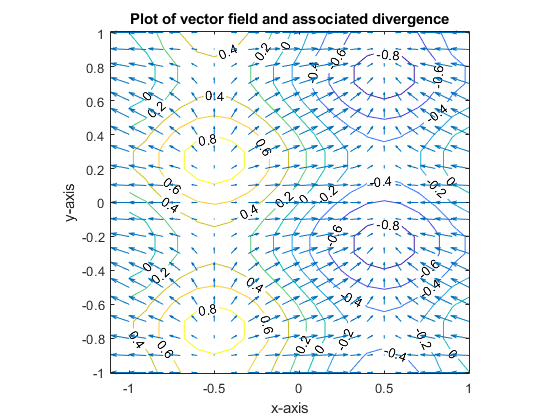
\includegraphics[width = 0.75 \textwidth]{./img/q1gi.png}
    \caption{Plot of vector field $\underline{u} = 2\cos\left(\pi x\right)\underline{i} + \sin^2\left(\pi y\right)\underline{j}$ and its associated divergence.}
\end{figure}
\lstset{language=Matlab,%
    %basicstyle=\color{red},
    breaklines=true,%
    morekeywords={matlab2tikz},
    keywordstyle=\color{blue},%
    morekeywords=[2]{1}, keywordstyle=[2]{\color{black}},
    identifierstyle=\color{black},%
    stringstyle=\color{mylilas},
    commentstyle=\color{mygreen},%
    showstringspaces=false,%without this there will be a symbol in the places where there is a space
    numbers=left,%
    numberstyle={\tiny \color{black}},% size of the numbers
    numbersep=9pt, % this defines how far the numbers are from the text
    emph=[1]{for,end,break},emphstyle=[1]\color{red}, %some words to emphasise
    %emph=[2]{word1,word2}, emphstyle=[2]{style},    
}
\lstinputlisting{./bin/q1gi.m}
\subsubsection{ii}
\begin{figure}[H]
    \centering
    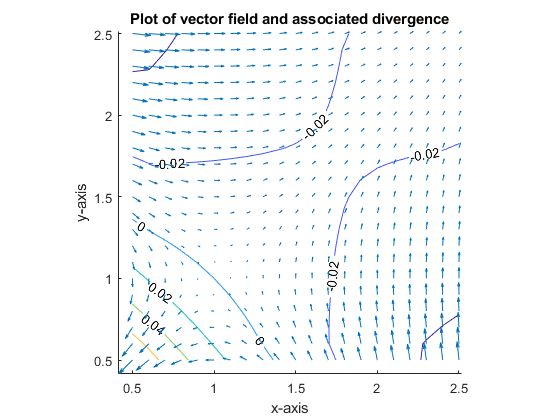
\includegraphics[width = 0.75 \textwidth]{./img/q1gii.png}
    \caption{Plot of vector field $\underline{u} = \ln\left(y\right)e^{-x}\underline{i} + \ln\left(x\right)e^{-y}\underline{j}$ and its associated divergence.}
\end{figure}
\lstset{language=Matlab,%
    %basicstyle=\color{red},
    breaklines=true,%
    morekeywords={matlab2tikz},
    keywordstyle=\color{blue},%
    morekeywords=[2]{1}, keywordstyle=[2]{\color{black}},
    identifierstyle=\color{black},%
    stringstyle=\color{mylilas},
    commentstyle=\color{mygreen},%
    showstringspaces=false,%without this there will be a symbol in the places where there is a space
    numbers=left,%
    numberstyle={\tiny \color{black}},% size of the numbers
    numbersep=9pt, % this defines how far the numbers are from the text
    emph=[1]{for,end,break},emphstyle=[1]\color{red}, %some words to emphasise
    %emph=[2]{word1,word2}, emphstyle=[2]{style},    
}
\lstinputlisting{./bin/q1gii.m}
\subsection{h}
\subsubsection{i}
\begin{figure}[H]
    \centering
    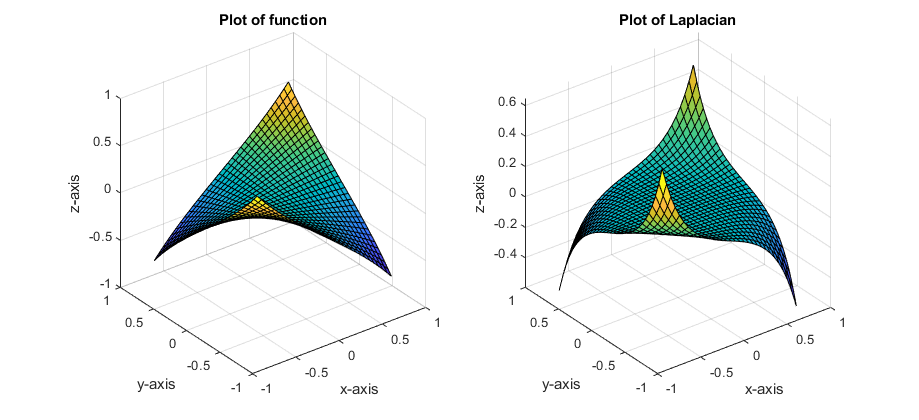
\includegraphics[width = \textwidth]{./img/q1hi.png}
    \caption{Plot of scalar function$z=\tan\left(xy\right)$ and its Laplacian.}
\end{figure}
\lstset{language=Matlab,%
    %basicstyle=\color{red},
    breaklines=true,%
    morekeywords={matlab2tikz},
    keywordstyle=\color{blue},%
    morekeywords=[2]{1}, keywordstyle=[2]{\color{black}},
    identifierstyle=\color{black},%
    stringstyle=\color{mylilas},
    commentstyle=\color{mygreen},%
    showstringspaces=false,%without this there will be a symbol in the places where there is a space
    numbers=left,%
    numberstyle={\tiny \color{black}},% size of the numbers
    numbersep=9pt, % this defines how far the numbers are from the text
    emph=[1]{for,end,break},emphstyle=[1]\color{red}, %some words to emphasise
    %emph=[2]{word1,word2}, emphstyle=[2]{style},    
}
\lstinputlisting{./bin/q1hi.m}
\subsubsection{ii}
\begin{figure}[H]
    \centering
    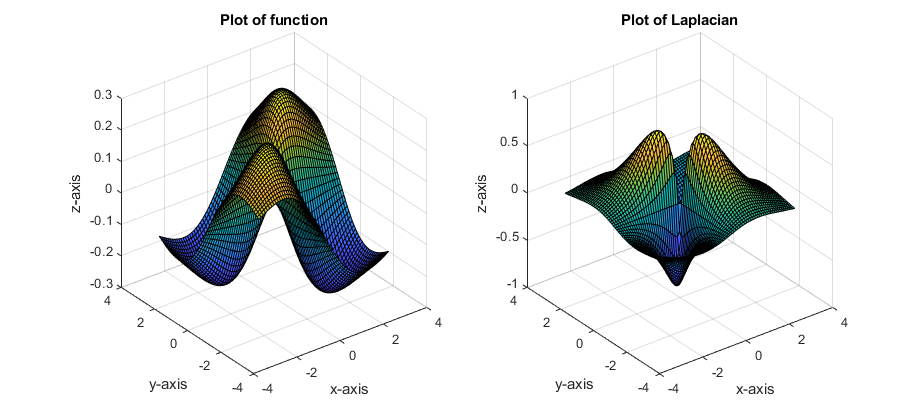
\includegraphics[width = \textwidth]{./img/q1hii.png}
    \caption{Plot of scalar function $z = xye^{-\sqrt{x^2 + y^2}}$ and its Laplacian.}
\end{figure}
\lstset{language=Matlab,%
    %basicstyle=\color{red},
    breaklines=true,%
    morekeywords={matlab2tikz},
    keywordstyle=\color{blue},%
    morekeywords=[2]{1}, keywordstyle=[2]{\color{black}},
    identifierstyle=\color{black},%
    stringstyle=\color{mylilas},
    commentstyle=\color{mygreen},%
    showstringspaces=false,%without this there will be a symbol in the places where there is a space
    numbers=left,%
    numberstyle={\tiny \color{black}},% size of the numbers
    numbersep=9pt, % this defines how far the numbers are from the text
    emph=[1]{for,end,break},emphstyle=[1]\color{red}, %some words to emphasise
    %emph=[2]{word1,word2}, emphstyle=[2]{style},    
}
\lstinputlisting{./bin/q1hii.m}
\section{Question 2}
\subsection{a}
In our series of equations, there are three unknown internal bar forces $N_{12}$, $N_{23}$, $N_{13}$, and three unknown reaction forces, $R_{2x}$, $R_{2y}$, $R_{3y}$. We also have two unknown angles, $\alpha$ and $\beta$, and the force $F$. Given that there are six unknowns that we would like to find and six equations with those variables, the conditions are fulfilled to solve this using matrices. Our answer would be in terms of the variables $\alpha$, $\beta$ and $F$. Values may be assumed for these or we can calculate them based on the geometry of the beams. 
\subsection{b}
\begin{gather}
    \begin{bmatrix}
        -\cos \alpha & \cos \beta & 0 & 0 & 0 & 0\\
        -\sin \alpha & -\sin \beta & 0 & 0 & 0 &0\\
        \cos \alpha & 1 & 0 & 1 & 0 & 0\\
        \sin \alpha & 0 & 0& 0 & 1 & 0\\
        0 & -\cos \beta & -1 & 0 & 0 & 0\\
        0 & \sin \beta & 0 & 0 & 0 & 1
    \end{bmatrix} \begin{bmatrix}
        N_{12}\\
        N_{13}\\
        N_{23}\\
        R_{2x}\\
        R_{2y}\\
        R_{3y}        
    \end{bmatrix} = \begin{bmatrix}
        0\\
        F\\
        0\\
        0\\
        0\\
        0\\
    \end{bmatrix}
\end{gather}
\subsection{c}
\lstset{language=Matlab,%
    %basicstyle=\color{red},
    breaklines=true,%
    morekeywords={matlab2tikz},
    keywordstyle=\color{blue},%
    morekeywords=[2]{1}, keywordstyle=[2]{\color{black}},
    identifierstyle=\color{black},%
    stringstyle=\color{mylilas},
    commentstyle=\color{mygreen},%
    showstringspaces=false,%without this there will be a symbol in the places where there is a space
    numbers=left,%
    numberstyle={\tiny \color{black}},% size of the numbers
    numbersep=9pt, % this defines how far the numbers are from the text
    emph=[1]{for,end,break},emphstyle=[1]\color{red}, %some words to emphasise
    %emph=[2]{word1,word2}, emphstyle=[2]{style},    
}
\lstinputlisting{./bin/q2c.m}
This returned the following:
\begin{gather}
    \begin{bmatrix}
        N_{12}\\
        N_{13}\\
        N_{23}\\
        R_{2x}\\
        R_{2y}\\
        R_{3y}        
    \end{bmatrix} = \begin{bmatrix}
        -800\\
        -600\\
        480\\
        0\\
        640\\
        360
    \end{bmatrix}
\end{gather}
\subsection{d}
\lstset{language=Matlab,%
    %basicstyle=\color{red},
    breaklines=true,%
    morekeywords={matlab2tikz},
    keywordstyle=\color{blue},%
    morekeywords=[2]{1}, keywordstyle=[2]{\color{black}},
    identifierstyle=\color{black},%
    stringstyle=\color{mylilas},
    commentstyle=\color{mygreen},%
    showstringspaces=false,%without this there will be a symbol in the places where there is a space
    numbers=left,%
    numberstyle={\tiny \color{black}},% size of the numbers
    numbersep=9pt, % this defines how far the numbers are from the text
    emph=[1]{for,end,break},emphstyle=[1]\color{red}, %some words to emphasise
    %emph=[2]{word1,word2}, emphstyle=[2]{style},    
}
\lstinputlisting{./bin/q2d.m}
This returned the following:
\begin{gather}
    \begin{bmatrix}
        N_{12}\\
        N_{13}\\
        N_{23}\\
        R_{2x}\\
        R_{2y}\\
        R_{3y}        
    \end{bmatrix} = \begin{bmatrix}
        -800\\
        -600\\
        480\\
        0\\
        640\\
        360
    \end{bmatrix}
\end{gather}
\subsection{e}
Matlab App Developer was utilised to create a user friendly interface for inputting the Force $F$, the lengths of each member (as shown in the diagram) and the coefficient matrix (where any mathematical expression can be inputted). The GUI displays the angles $\alpha$ and $\beta$ as well as a table of values for each of the internal bar and reaction forces. The code is shown below.
\lstset{language=Matlab,%
    %basicstyle=\color{red},
    breaklines=true,%
    morekeywords={matlab2tikz},
    keywordstyle=\color{blue},%
    morekeywords=[2]{1}, keywordstyle=[2]{\color{black}},
    identifierstyle=\color{black},%
    stringstyle=\color{mylilas},
    commentstyle=\color{mygreen},%
    showstringspaces=false,%without this there will be a symbol in the places where there is a space
    numbers=left,%
    numberstyle={\tiny \color{black}},% size of the numbers
    numbersep=9pt, % this defines how far the numbers are from the text
    emph=[1]{for,end,break},emphstyle=[1]\color{red}, %some words to emphasise
    %emph=[2]{word1,word2}, emphstyle=[2]{style},    
}
\lstinputlisting{./bin/q2eApp_exported.m}
\begin{figure}[H]
    \centering
    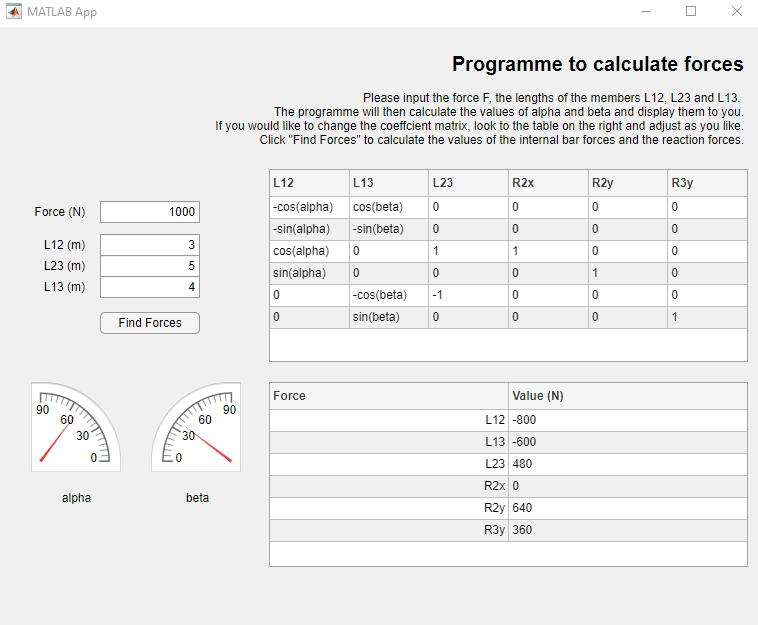
\includegraphics[width = 0.75 \textwidth]{./img/q2e.png}
    \caption{Screenshot from Matlab App, showcasing GUI, input and output parameters.}
\end{figure}
\subsection{f}
Code was written to generate a table of data:
\lstset{language=Matlab,%
    %basicstyle=\color{red},
    breaklines=true,%
    morekeywords={matlab2tikz},
    keywordstyle=\color{blue},%
    morekeywords=[2]{1}, keywordstyle=[2]{\color{black}},
    identifierstyle=\color{black},%
    stringstyle=\color{mylilas},
    commentstyle=\color{mygreen},%
    showstringspaces=false,%without this there will be a symbol in the places where there is a space
    numbers=left,%
    numberstyle={\tiny \color{black}},% size of the numbers
    numbersep=9pt, % this defines how far the numbers are from the text
    emph=[1]{for,end,break},emphstyle=[1]\color{red}, %some words to emphasise
    %emph=[2]{word1,word2}, emphstyle=[2]{style},    
}
\lstinputlisting{./bin/q2f.m}
\begin{table}[H]
    \centering
    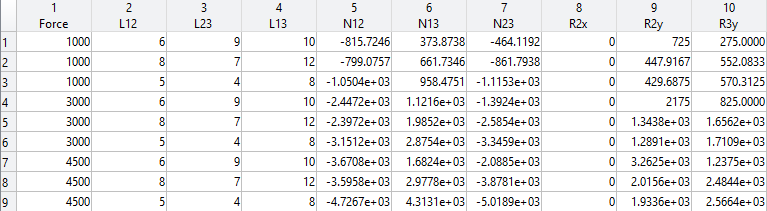
\includegraphics[width = \textwidth]{./img/q2f.png}
    \caption{Table of data generated from MATALB, showing forces in three configuration with three different loads.}
\end{table}
\begin{table}[H]
    \centering
    \begin{tabular}{llllllllll}
        \toprule
        Force & L12 & L13 & L23 & N13 & N23 & N13 & R2x & R2y & R3y\\
        (\si{\newton}) & (\si{\metre}) & & & (\si{\newton}) & & & & \\
        \midrule
        1000 & 6 & 9 & 10 & -815.7  & 373.9  & -464.1  & 0 & 725.0  & 275.0  \\
        1000 & 8 & 7 & 12 & -799.1  & 661.7  & -861.8  & 0 & 447.9  & 552.1  \\
        1000 & 5 & 4 & 8  & -1050.4 & 958.5  & -1115.3 & 0 & 429.7  & 570.3  \\
        3000 & 6 & 9 & 10 & -2447.2 & 1121.6 & -1392.4 & 0 & 2175.0 & 825.0  \\
        3000 & 8 & 7 & 12 & -2397.2 & 1985.2 & -2585.4 & 0 & 1343.8 & 1656.3 \\
        3000 & 5 & 4 & 8  & -3151.2 & 2875.4 & -3346.0 & 0 & 1289.1 & 1710.9 \\
        4500 & 6 & 9 & 10 & -3670.8 & 1682.4 & -2088.5 & 0 & 3262.5 & 1237.5 \\
        4500 & 8 & 7 & 12 & -3595.8 & 2977.8 & -3878.1 & 0 & 2015.6 & 2484.4 \\
        4500 & 5 & 4 & 8  & -4726.7 & 4313.1 & -5018.9 & 0 & 1933.6 & 2566.4 \\
        \bottomrule
    \end{tabular}
    \caption{Table to show values of internal bar forces and reaction forces.}
\end{table}
\section{Question 3}
\lstset{language=Matlab,%
    %basicstyle=\color{red},
    breaklines=true,%
    morekeywords={matlab2tikz},
    keywordstyle=\color{blue},%
    morekeywords=[2]{1}, keywordstyle=[2]{\color{black}},
    identifierstyle=\color{black},%
    stringstyle=\color{mylilas},
    commentstyle=\color{mygreen},%
    showstringspaces=false,%without this there will be a symbol in the places where there is a space
    numbers=left,%
    numberstyle={\tiny \color{black}},% size of the numbers
    numbersep=9pt, % this defines how far the numbers are from the text
    emph=[1]{for,end,break},emphstyle=[1]\color{red}, %some words to emphasise
    %emph=[2]{word1,word2}, emphstyle=[2]{style},    
}
\lstinputlisting{./bin/q3a.m}
\begin{table}[H]
    \centering
    \begin{tabular}{lll}
        \toprule
        & \textbf{A} & \textbf{B}\\
        \midrule
        Mean & 50991.90 & 50328.27\\
        Standard Deviation & 53.77 & 863.99\\
        \bottomrule
    \end{tabular}
    \caption{Table to show values of means and standard deviations of weekly output of vaccines for manufacturer A and B.}
\end{table}
\subsection{b}
Hypothesis test for efficiency. We can use a two-tailed binomial distribution for this test. A two-tailed test applies here as we are testing for a difference between the efficiencies of each manufacturer. \begin{itemize}
    \item Null hypothesis - the efficiencies for both manufacturers are the same.
    \item Alternate hypothesis - the efficiencies for both manufacturers are not the same.
\end{itemize}
\begin{align}
    H_0: \; P_a - P_b = 0\\
    H_1: \; P_a - P_b \neq 0
\end{align}
Hypothesis test for factory output. As we do not know the true population standard deviation, we can utilise a two-tailed t-test. As for the efficiency test, a two-tailed test is used as we are testing for a difference between the two manufacturer's weekly output.
\begin{itemize}
    \item Null hypothesis - the weekly outputs for both manufacturers are the same.
    \item Alternate hypothesis - the weekly outputs for both manufacturers are not the same.
\end{itemize}
\begin{align}
    H_0: \; \mu_a - \mu_b = 0\\
    H_1: \; \mu_a - \mu_b \neq 0 
\end{align}
\subsection{c}
Test for efficiency. As our sample sizes are larger than 25, we can assume a normal distribution applies and utilise Z-values. Finding total proportion:
\begin{gather}
    \hat{p}_A = 0.94 \hspace{1cm} \hat{p}_B = 0.92\\
    \hat{p}_T = \frac{n_A \hat{p}_A + n_B \hat{p}_B}{n_A + n_B}\\
    \hat{p}_T = \frac{0.94\cdot 2000 + 0.92 \cdot 500}{2000 + 500}\\
    \hat{p}_T = 0.936
\end{gather}
The corresponding Z-value is ($P_a - P_b = 0$):
\begin{gather}
    Z^* = \frac{\left(\hat{p}_A - \hat{p}_B\right) - \left(p_A - p_B\right)}{\sqrt{\hat{p}_T \left(1-\hat{p}_T\right)\left(\frac{1}{n_A} + \frac{1}{n_B}\right)}}\\
    Z^* = \frac{0.94 -0.92 - 0}{\sqrt{0.936 \left(1-0.936\right)\left(\frac{1}{2000} + \frac{1}{500}\right)}} = 1.634
\end{gather}
At 5\% significance in a two-tailed test, our critical Z-value is 1.96:
\begin{eqnarray}
    Z^* = 1.634 < Z^*_{crit} = 1.96
\end{eqnarray}
We found our Z-value to be smaller than the critical value, hence there is not sufficient data to reject the null hypothesis and there is 95\% confidence that the efficiencies of the vaccine outputs are the same for both manufacturers. 

Test for weekly output. As our sample sizes are larger than 25, we can assume a normal distribution applies and utilise Z-values ($\mu_a - \mu_b = 0$):
\begin{gather}
    Z^* = \frac{\left(\hat{x}_A - \hat{x}_R\right)-\left(\mu_A - \mu_R\right)}{\sqrt{\frac{s_A^2}{n_A} + \frac{s_B^2}{n_B}}}\\
    Z^* = \frac{50991.9 - 50328.27 - 0}{\sqrt{\frac{53.77^2}{30} + \frac{863.99^2}{30}}} = 4.199
\end{gather}
At 5\% significance in a two-tailed test, our critical Z-value is 1.96:
\begin{equation}
    Z^* = 4.199 > Z^*_{crit/\frac{\alpha}{2}} = 1.96
\end{equation} 
The Z-value for the weekly output is higher than the critical value, hence there is sufficient evidence to reject the null hypothesis and there is a 95\% confidence that the weekly outputs are different for both manufacturers. The mean weekly output of manufacturer A is larger than B, hence we can say that the weekly output of A is larger than B. For a one tail test ($\mu_A - \mu_B > 0$), our $Z^*_{crit}$ value would be lower than that of a two-tailed test at 5\% significance.
\section{Question 4}
\subsection{a}
\subsubsection{i}
Let $X$ be number of trials until the first head appears. Coin is unbiased, thus $X \sim Geo\left(\frac{1}{2}\right)$.
\begin{align}
    P(X = 1) &= \frac{1}{2}\\
    P(X = 2) &= \frac{1}{2}\cdot\frac{1}{2} = \frac{1}{4}\\
    P(X = 3) &= \frac{1}{2}\cdot\frac{1}{2}\cdot\frac{1}{2} = \frac{1}{8}\\
    P(X = n) &= \frac{1}{2^n}
\end{align}
\subsubsection{ii}
\begin{gather}
    \sum_{n=1}^{\infty} P(X=n) = \frac{1}{2} + \frac{1}{4} + \frac{1}{8} + ... + \frac{1}{2^n}
\end{gather}
Geometric series, hence:
\begin{gather}
    a = \frac{1}{2}, \, r = \frac{1}{2}\\
    \sum_{n=1}^{\infty} P(X=n) = \frac{a}{1-r} = \frac{\frac{1}{2}}{1-\frac{1}{2}} = 1
\end{gather}
\subsection{b}
\begin{equation}
    f(x) = \begin{cases}
        \alpha \left(1 - x^2\right)\\
        0 
    \end{cases} \begin{array}{l}
        -1 \leq x \leq 1\\
        \textrm{otherwise}
    \end{array}
\end{equation}
\subsubsection{i}
Area under the probability density function equals to 1, hence area under the integral also equals to 1: 
\begin{align}
    F(x) = 1 &= \int_{-1}^1 \left(\alpha - \alpha x^2\right) \dif x\\
    &= \left[\alpha x - \frac{\alpha x^3}{3}\right]_{-1}^{1}\\
    &= \left(\alpha - \frac{\alpha}{3} + \alpha -\frac{\alpha}{3} \right)\\
    \frac{4\alpha}{3} &= 1\\
    \alpha &= \frac{3}{4}
\end{align}
$P\left(-\frac{1}{2} \leq x \leq \frac{1}{2} \right)$
\begin{align}
    P\left(-\frac{1}{2} \leq x \leq \frac{1}{2} \right) &= \int_{-\frac{1}{2}}^{\frac{1}{2}} \left(\frac{3}{4} - \frac{3x^2}{4}\right) \dif x\\
    &= \left[\frac{3x}{4} - \frac{x^3}{4}\right]_{-\frac{1}{2}}^{\frac{1}{2}}\\
    &= \left(\frac{3}{8} - \frac{1}{32} + \frac{3}{8} - \frac{1}{32} \right)\\
    &= \frac{11}{16}\\
    &= 68.75\%
\end{align}
$P\left(\frac{1}{4} \leq x \leq 2 \right)$
\begin{align}
    P\left(\frac{1}{4} \leq x \leq 2 \right) &= \int_{\frac{1}{4}}^{1} \left(\frac{3}{4} - \frac{3x^2}{4}\right) \dif x\\
    &= \left[\frac{3x}{4} - \frac{x^3}{4}\right]_{\frac{1}{4}}^{1}\\
    &= \left(\frac{3}{4} - \frac{1}{4} - \frac{3}{16} + \frac{1}{256} \right)\\
    &= \frac{81}{256}\\
    &= 31.64\%
\end{align}
\subsubsection{ii}
$P(X \leq x) = 0.95$
\begin{align}
    P(X \leq x) = 0.95 &= \int_{-1}^{x} \left(\frac{3}{4} - \frac{3x^2}{4}\right) \dif x\\
    \left[\frac{3x}{4} - \frac{x^3}{4}\right]_{-1}^{x} &= 0.95 \\
    \left(\frac{3x}{4} - \frac{x^3}{4} + \frac{3}{4} - \frac{1}{4} \right) &= 0.95\\
    \frac{x^3}{4} -\frac{3x}{4} + \frac{9}{20} &= 0
\end{align}
Solving via calculator and rejecting values outside the range of $-1 \leq x \leq 1$:
\begin{align}
    x_1 &\neq 1.2481\\
    x_2 &\neq -1.9777\\
    x_3 &= 0.7293
\end{align}
\subsection{c}
\subsubsection{i}
$X$ and $Y$ are independent in the case the following equation is satisfied:
\begin{equation}
    f(x,y) = f(x) f(y)
\end{equation}
We can express the probability density function as:
\begin{equation}
    f(x,y) = \alpha e^{-0.1\left(x+y\right)} = \left(be^{-0.1x}\right)\left(ce^{-0.1y}\right)
\end{equation}
where $b\cdot c = \alpha$.
\begin{gather}
    f_1(x) = be^{-0.1x} \textrm{ and } f_2(y) = ce^{-0.1y}\\
    \alpha e^{-0.1\left(x+y\right)} = \left(be^{-0.1x}\right)\left(ce^{-0.1y}\right)\\
    f(x,y) = f_1(x)f_2(y)
\end{gather}
Conditions are satisfied, hence $X$ and $Y$ are independent.
\subsubsection{ii}
Area under probability density function equals to 1:
\begin{align}
    F(x,y) = 1 &= \lim_{t\rightarrow \infty} \int_{y=0}^{t} \int_{x=0}^{t} \left(\alpha e^{-0.1\left(x+y\right)}\right) \dif x \dif y\\
    &= \lim_{t\rightarrow \infty} \int_{y=0}^{t} \left[ -\frac{\alpha}{0.1} e^{-0.1\left(x+y\right)} \right]_{x=0}^t \dif y\\
    &= \lim_{t\rightarrow \infty} \int_{y=0}^{t} \left(\frac{\alpha}{0.1} e^{-0.1y} \right) \dif y\\
    &= \lim_{t\rightarrow \infty} \left[ -\frac{\alpha}{0.01} e^{-0.1y} \right]_{y=0}^t\\
    &= 0 + \frac{\alpha}{0.01}e^{0}\\
    \frac{\alpha}{0.01} &= 1\\
    \alpha &= 0.01
\end{align}
The marginal distributions for $x$ can be found as:
\begin{align}
    F(x) &= b \lim_{t\rightarrow \infty} \int_0^t\left(e^{-0.1x}\right)\dif x = \left[b\left(-10 e^{-0.1x}\right)\right]_0^t\\
    1 &= b\left(0 + 10\right) = 10b \\
    b &= 0.1
\end{align}
Therefore:
\begin{equation}
    f_1(x) = \begin{cases}
        0.1e^{-0.1x}\\
        0
    \end{cases} \begin{array}{l}
        x > 0\\
        x \leq 0
    \end{array}
\end{equation}
We also know that $b\cdot c = \alpha$, hence:
\begin{gather}
    b = 0.1 \hspace{1cm} c = 0.1\\
    f_2(y) = \begin{cases}
        0.1e^{-0.1y}\\
        0
    \end{cases} \begin{array}{l}
        y > 0\\
        y \leq 0
    \end{array}
\end{gather}
\subsubsection{iii}
$P(X \geq 10)$
\begin{align}
    P(X \geq 10) &= \lim_{t\rightarrow \infty} \int_{x=10}^{t} \int_{y=0}^{t} \left(0.01 e^{-0.1\left(x + y\right)}\right) \dif y \dif x\\
    &= \lim_{t\rightarrow \infty} \int_{x=10}^{t} \left[-0.1 e^{-0.1\left(x + y\right)}\right]_{y=0}^t \dif x\\
    &= \lim_{t\rightarrow \infty} \int_{x=10}^{t} \left[0+0.1 e^{-0.1x}\right] \dif x\\
    &= \lim_{t\rightarrow \infty} \left[- e^{-0.1x}\right]_{10}^t\\
    &= \left[0 + e^{-1}\right]\\
    &= 0.3679 = 36.79\%
\end{align}
\subsubsection{iv}
$P(y < x)$
\begin{align}
    P(y < x) &= \lim_{t\rightarrow \infty} \int_{x=0}^{t} \int_{y=0}^{x} \left(0.01 e^{-0.1\left(x + y\right)}\right) \dif y \dif x\\
    &= \lim_{t\rightarrow \infty} \int_{x=0}^{t} \left[-0.1 e^{-0.1\left(x + y\right)}\right]_{y=0}^x \dif x\\
    &= \lim_{t\rightarrow \infty} \int_{x=0}^{t} \left(-0.1e^{-0.2x}+0.1 e^{-0.1x}\right) \dif x\\
    &= \lim_{t\rightarrow \infty} \left[0.5 e^{-0.2x}- e^{-0.1x}\right]_{0}^t\\
    &= \left[0 - 0 - 0.5 + 1\right]\\
    &= 0.5 = 50\%
\end{align}
\end{document}